\documentclass[a4paper,onecolumn,oneside,12pt,extrafontsizes]{article}
\usepackage[utf8]{inputenc}
\usepackage[T1]{fontenc}
\usepackage{lmodern}
\usepackage[polish]{babel}
\usepackage{graphicx}
\usepackage{hyperref}
\author{Kamil Kasjan 230211}
\title{Modelowanie i Identyfikacja - sprawozdanie I}

\begin{document}
\maketitle

\section{Generatory liczb o rozkładzie jednostajnym}
W trakcie zajęć laboratoryjnych należało zaimplementować 3 generatory:
\begin{enumerate}
	\item{sinusoidalny}
	\item{piłokształtny}
	\item{fibonacciego}
\end{enumerate}
Po zaimplementowaniu, celem sprawdzenia rzeczywistego rozkładu prawdopodobieństwa wygenerowanych zmiennych narysowano histogram, oraz przeprowadzono test $Chi^2$. 
\begin{figure}[!htb]
	\centering
	\caption{Histogramy zmiennych wygenerowanych przez zadane generatory}
	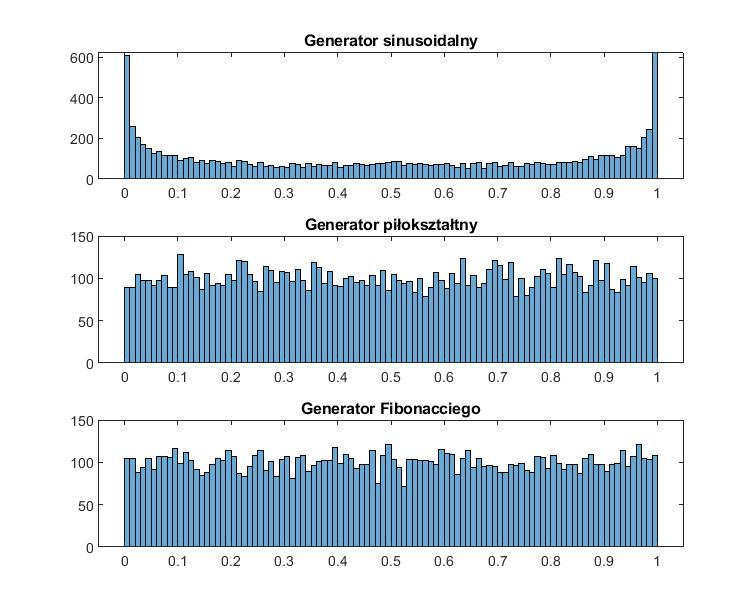
\includegraphics[width=9cm]{fig1.jpg}
\end{figure}
\newpage

Zmienne generowane przy użyciu generatorów piłokształtnego i Fibonacciego faktycznie były zmiennymi o rozkładzie jednostajnym, co potwierdził test $Chi^2$. Generator sinusoidalny nie dawał takich rezultatów co wynika z faktu, że funkcja sinus jest odcinkami szybkozmienna, przez co istnieje większe prawdopodobieństwo, że argumentem kolejnej iteracji będzie wartość skrajnie mała lub skrajnie duża, co można zaobserwować na histogramie. Punkty startowe za każdym razem były generowane za pomocą funkcji rand, dzięki czemu można było uzyskać różne wyniki. W specyficznych przypadkach mogło się zdarzyć, że częstotliwość funkcji sinus(x) i funkcji saw(x) były tak dobrane, że przy wygenerowanym punkcie startowym generator za każdym razem generował tę samą wartość.
\section{Metoda odwrotnej dystrybuanty}
Kolejnym zadaniem było zaimplementowanie generatorów, które generowały zmienne losowe o zadanej gęstości za pomocą metody odwrotnej dystrybuanty bazując na zmiennych o rozkładzie jednostajnym. W tym celu należało analitycznie scałkować funkcję gęstości celem otrzymania dystrybuanty i wynikową funkcję odwrócić. Aby otrzymać zmienne losowe o żądanej gęstości prawdopodobieństwa trzeba było za argumenty funkcji wynikowej podstawić zmienne o rozkładzie jednostajnym.
\begin{figure}[!htb]
	\centering
	\caption{Histogramy zmiennych wygenerowanych metodą odwrotnej dystrybuanty}
	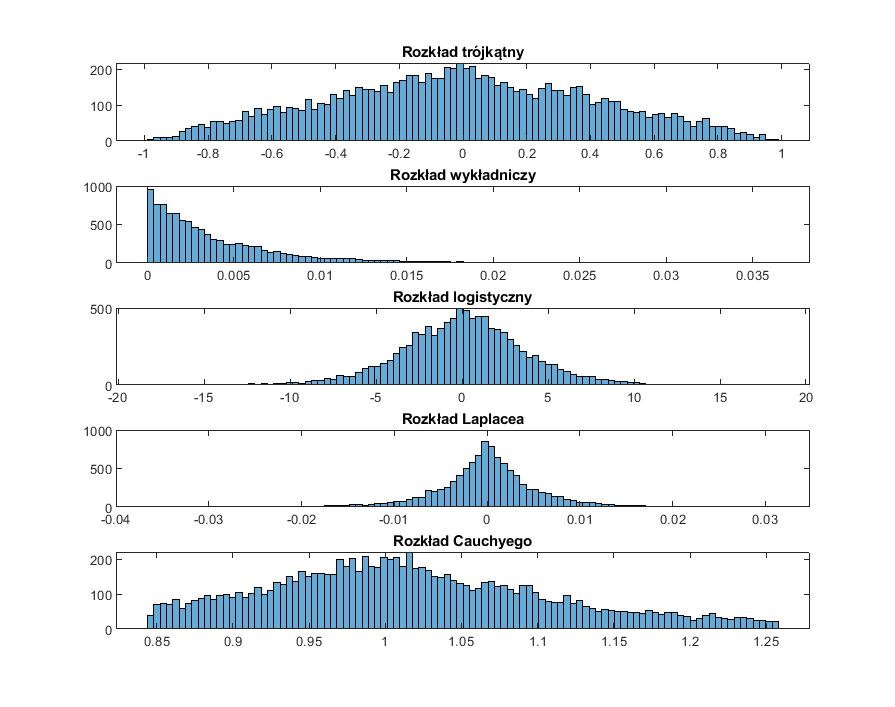
\includegraphics[width=10cm]{fig2.jpg}
\end{figure}
\newpage

Dla każdego generatora wykonano test Kołmogorowa-Smirnowa. We wszystkich przypadkach test dał wynik 0, co potwierdza poprawność działania generatorów.
\subsection{Wnioski}
Niewątpliwą zaletą tej metody jest mała złożoność obliczeniowa. Niestety jest to obarczone koniecznością ręcznego obliczenia analitycznej postaci funkcji, co nie zawsze jest proste tudzież możliwe. Problem ten można jednak obejść wykorzystując metody numerycznego całkowania i odwracania funkcji, co zwiększa złożoność obliczeniową, ale pozwala na bezstratne wygenerowanie zmiennych losowych o w zasadzie dowolnym rozkładzie prawdopodobieństwa.
\section{Metoda eliminacji}
W tej metodzie zmienne o zadanym rozkładzie generuje się z wykorzystaniem dwóch zmiennych o rozkładzie jednostajnym. Żądaną funkcję gęstości podaje się analitycznie, następnie ogranicza się płaszczyznę, na której generowane są zmienne losowe za pomocą funkcji ograniczającej (jej dobór zależy od przypadku i wpływa na ilość próbek odrzuconych). W kolejnym kroku wygenerowaną dwuwymiarową zmienną porównuje się z funkcją ograniczającą i jeżeli warunek jest spełniony, to próbka jest przyjmowana. W przeciwnym wypadku odrzucana. 

Z wykorzystaniem tej metody wygenerowano zmienne losowe zadanych rozkładach:
\begin{enumerate}
	\item{zadanym krzywą łamaną}
	\item{normalnym ograniczonym krzywą rozkładu wykładniczego}
	\item{normalnym ograniczonym krzywą rozkłądu Laplace'a}
	\item{zadanym parabolą}
\end{enumerate}

Rozkłady ograniczono takimi funkcjami, aby liczba próbek zaakceptowanych była większa niż odrzuconych. W przypadku rozkładu zadanego parabolą, ponieważ liczby są losowane nie z zakresu liczb rzeczywistych a określonego przedziału, zastosowano ograniczenie w formie rozkładu jednostajnego przemnożonego przez stałą równą wartości funkcji gęstości w punkcie 0.

Dla wygenerowanych rozkładów przeprowadzono test Kołmogorowa-Smirnowa, który we wszystkich przypadkach zwrócił wartość 0, czyli potwierdził prawidłowość uzyskanych wyników.

\newpage 
\begin{figure}[!htb]
	\centering
	\caption{Rozkład zadany krzywą łamaną, ograniczony rozkładem jednostajnym}
	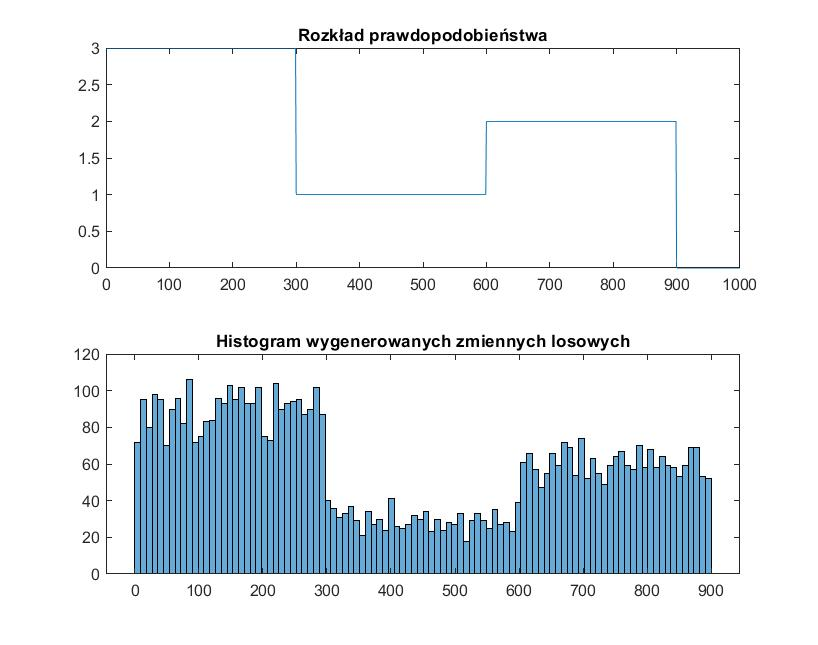
\includegraphics[width=9cm]{fig3.jpg}
\end{figure}

\begin{figure}[!htb]
	\centering
	\caption{Rozkład normalny ograniczony rozkładem wykładniczym przemnożonym przez stałą $\sqrt{\frac{2e}{\pi}}$ }
	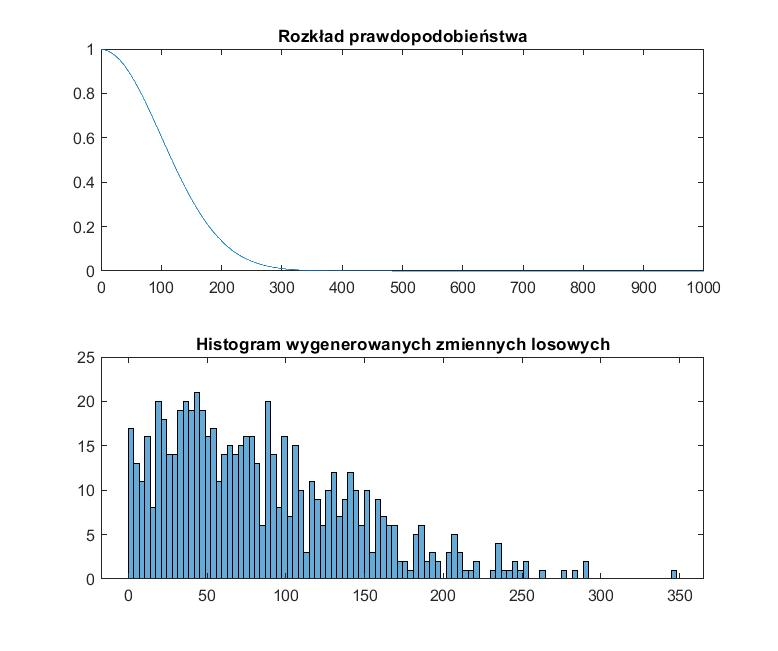
\includegraphics[width=9cm]{fig4.jpg}
\end{figure}

\begin{figure}[!htb]
	\centering
	\caption{Rozkład normalny ograniczony rozkładem Laplace'a przemnożonym przez stałą $\sqrt{\frac{2e}{\pi}}$ }
	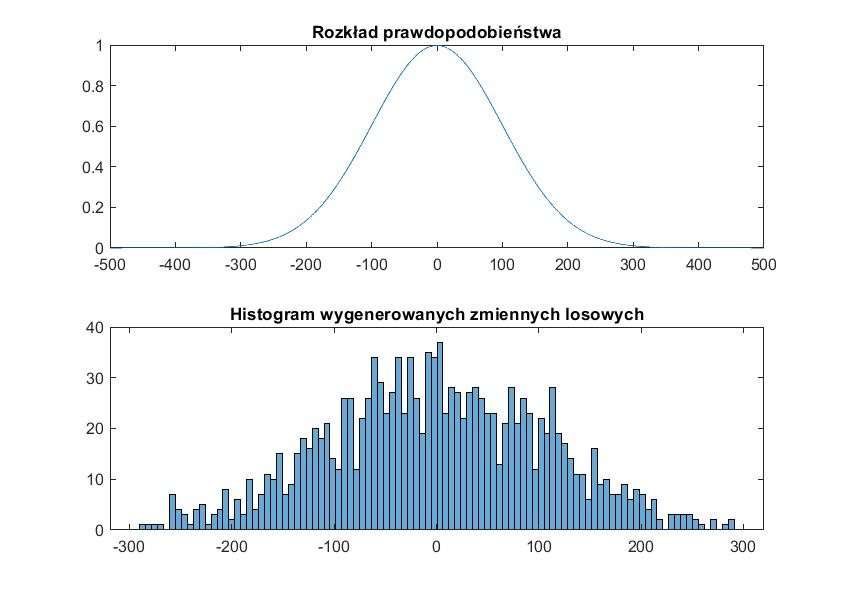
\includegraphics[width=9cm]{fig5.jpg}
\end{figure}

\begin{figure}[!htb]
	\centering
	\caption{Rozkład zadany parabolą ograniczony rozkładem jednostajnym przemnożonym przez stałą 4.5}
	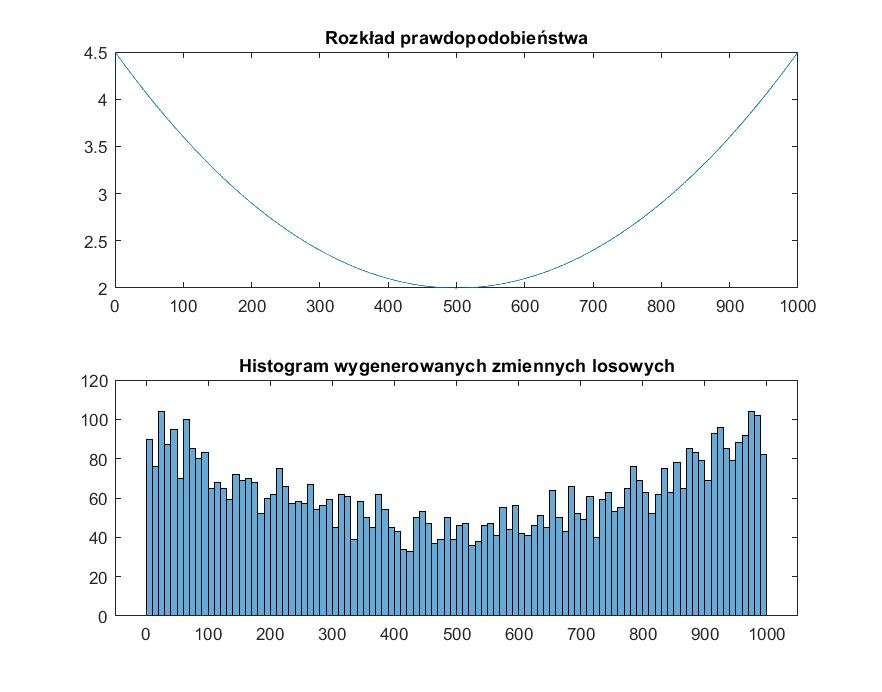
\includegraphics[width=9cm]{fig6.jpg}
\end{figure}
\newpage
\newpage
\subsection{Wnioski}
Metoda eliminacji w przeciwieństwie do metody odwrotnej dystrybuanty jest bardziej kosztowna pod względem obliczeń przez wzgląd na odrzucanie części próbek. Dobór funkcji ograniczającej jest istotny z punktu widzenia minimalizacji strat próbek. Mimo stratności, dużą zaletą tej metody jest możliwość wygenerowania zmiennych losowych o dowolnym rozkładzie.

\section{Kody źródłowe}
\href{https://github.com/waniadze314/Modelowanie_i_Identyfikacja}{Link do repozytorium GitHub}
\end{document}